%% FEUP THESIS STYLE for LaTeX2e
%% how to use feupteses (English version)
%%
%% FEUP, JCL & JCF, 31 July 2012
%%
%% PLEASE send improvements to jlopes at fe.up.pt and to jcf at fe.up.pt
%%

%%========================================
%% Commands: pdflatex meic_thesis
%%           bibtex meic_thesis
%%           makeindex meic_thesis (only if creating an index)
%%           pdflatex meic_thesis
%% Alternative:
%%           latexmk -pdf meic_thesis.tex
%% Using the Makefile:
%%           make
%%========================================

%% 2021-07-20: One-sided output by default
\documentclass[11pt,a4paper]{report}
%% For two-sided printing (for dead-tree output) comment previous line
%% and uncomment the next line
%\documentclass[11pt,a4paper,twoside,openright]{report}

%% For iso-8859-1 (latin1), comment next line and uncomment the second line
\usepackage[utf8]{inputenc}
%\usepackage[latin1]{inputenc}

%% English version

%% MEIC options
\usepackage[meic]{feupteses}                  % work version
%\usepackage[meic,juri]{feupteses}             % jury version
%\usepackage[meic,final]{feupteses}            % final version
%\usepackage[meic,final,onpaper]{feupteses}    % final on paper version

%% Additional options for feupteses.sty: 
%% - portugues: titles, etc in portuguese
%% - onpaper: links are not shown (for paper versions)
%% - backrefs: include back references from bibliography to citation place

%% Uncomment the next lines if side by side graphics used
\usepackage[lofdepth,lotdepth]{subfig}
\usepackage{graphicx}
\usepackage{float}

% Listings
\definecolor{cloudwhite}{cmyk}{0,0,0,0.025}  % color

%% Include source-code listings package
\usepackage{listings}
\lstset{ %
 language=C,                        % choose the language of the code
 basicstyle=\footnotesize\ttfamily,
 keywordstyle=\bfseries,
 numbers=left,                      % where to put the line-numbers
 numberstyle=\scriptsize\texttt,    % the size of the fonts that are used for the line-numbers
 stepnumber=1,                      % the step between two line-numbers. If it's 1 each line will be numbered
 numbersep=8pt,                     % how far the line-numbers are from the code
 frame=tb,
 float=htb,
 aboveskip=8mm,
 belowskip=4mm,
 backgroundcolor=\color{cloudwhite},
 showspaces=false,                  % show spaces adding particular underscores
 showstringspaces=false,            % underline spaces within strings
 showtabs=false,                    % show tabs within strings adding particular underscores
 tabsize=2,                         % sets default tabsize to 2 spaces
 captionpos=b,                      % sets the caption-position to bottom
 breaklines=true,                   % sets automatic line breaking
 breakatwhitespace=false,           % sets if automatic breaks should only happen at whitespace
 escapeinside={\%*}{*)},            % if you want to add a comment within your code
 morekeywords={*,var,template,new}  % if you want to add more keywords to the set
}

% Todo notes package
\usepackage{todonotes}
\usepackage{xcolor}
\presetkeys%
    {todonotes}%
    {inline,backgroundcolor=yellow}{}


%%Uncomment to create an index (at the end of the document)
%\makeindex

%% Path to the figures directory
%% TIP: use folder ``figures'' to keep all your figures
\graphicspath{{figures/}}

%%----------------------------------------
%% TIP: if you want to define more macros, use an external file to keep them
%some macro definitions

% format
\newcommand{\class}[1]{{\normalfont\slshape #1\/}}

% entities
\newcommand{\Feup}{Faculdade de Engenharia da Universidade do Porto}

\newcommand{\svg}{\class{SVG}}
\newcommand{\scada}{\class{SCADA}}
\newcommand{\scadadms}{\class{SCADA/DMS}}

%%----------------------------------------

%%========================================
%% Start of document
%%========================================
\begin{document}

%%----------------------------------------
%% Information about the work
%%----------------------------------------
\title{Improving the Developer Experience of Dockerfiles}
\author{João Pereira da Silva Matos}

%% Comment next line if not necessary for degree
%\degree{Programa Doutoral em Engenharia Informática}

%% Uncomment next line for date of submission
%\thesisdate{July 31, 2008}

%% Comment next line copyright text if not used
%\copyrightnotice{Name of the Author, 2008}

\supervisor{Supervisor}{Prof.\ Filipe Correia}

%% Uncomment next line if necessary
%\supervisor{Second Supervisor}{Prof.\Name of the Supervisor}

%% Uncomment committee stuff in the final version
%\committeetext{Approved in oral examination by the committee:}
%\committeemember{President}{Prof.\ Name of the President}
%\committeemember{Referee}{Prof.\ Name of the Referee}
%\committeemember{Referee}{Prof.\ Name of the Referee}

%\committeetext{Aprovado em provas públicas pelo Júri:}
%\committeemember{Presidente}{Prof.\ Nome do presidente do júri}
%\committeemember{Arguente}{Prof.\ Nome do arguente do júri}
%\committeemember{Vogal}{Prof.\ Nome do vogal do júri}

%% Uncomment signature line in the final on paper version if used
%\signature

%% Specify cover logo (in folder ``figures'')
\logo{uporto-feup.pdf}

%% Uncomment next line for additional text below the author's name (front page)
% \additionalfronttext{Preparação da Dissertação}
%\additionalfronttext{Dissertation Planning}

%%----------------------------------------
%% Preliminary materials
%%----------------------------------------

% remove unnecessary \include{} commands
\begin{Prolog}
  % \chapter*{Resumo}
%\addcontentsline{toc}{chapter}{Resumo}

Este documento ilustra o formato a usar em dissertações na \Feup.
São dados exemplos de margens, cabeçalhos, títulos, paginação, estilos
de índices, etc. 
São ainda dados exemplos de formatação de citações, figuras e tabelas,
equações, referências cruzadas, lista de referências e índices.
Este documento não pretende exemplificar conteúdos a usar. 
É usado o \emph{Loren Ipsum} para preencher a dissertação.

Lorem ipsum dolor sit amet, consectetuer adipiscing elit. Etiam vitae
quam sed mauris auctor porttitor. Mauris porta sem vitae arcu sagittis
facilisis. Proin sodales risus sit amet arcu. Quisque eu pede eu elit
pulvinar porttitor. Maecenas dignissim tincidunt dui. Pellentesque
habitant morbi tristique senectus et netus et malesuada fames ac
turpis egestas. Donec non augue sit amet nulla gravida
rutrum. Vestibulum ante ipsum primis in faucibus orci luctus et
ultrices posuere cubilia Curae; Nunc at nunc. Etiam egestas. 

Donec malesuada pede eget nunc. Fusce porttitor felis eget mi mattis
vestibulum. Pellentesque faucibus. Cras adipiscing dolor quis
mi. Quisque sagittis, justo sed dapibus pharetra, lectus velit
tincidunt eros, ac fermentum nulla velit vel sapien. Vestibulum sem
mauris, hendrerit non, feugiat ac, varius ornare, lectus. Praesent
urna tellus, euismod in, hendrerit sit amet, pretium vitae,
nisi. Proin nisl sem, ultrices eget, faucibus a, feugiat non,
purus. Etiam mi tortor, convallis quis, pharetra ut, consectetuer eu,
orci. Vivamus aliquet. Aenean mollis fringilla erat. Vivamus mollis,
purus at pellentesque faucibus, sapien lorem eleifend quam, mollis
luctus mi purus in dui. Maecenas volutpat mauris eu lectus. Morbi vel
risus et dolor bibendum malesuada. Donec feugiat tristique erat. Nam
porta auctor mi. Nulla purus. Nam aliquam. 


\chapter*{Abstract}
%\addcontentsline{toc}{chapter}{Abstract}

Here goes the abstract written in English.

Lorem ipsum dolor sit amet, consectetuer adipiscing elit. Sed vehicula
lorem commodo dui. Fusce mollis feugiat elit. Cum sociis natoque
penatibus et magnis dis parturient montes, nascetur ridiculus
mus. Donec eu quam. Aenean consectetuer odio quis nisi. Fusce molestie
metus sed neque. Praesent nulla. Donec quis urna. Pellentesque
hendrerit vulputate nunc. Donec id eros et leo ullamcorper
placerat. Curabitur aliquam tellus et diam. 

Ut tortor. Morbi eget elit. Maecenas nec risus. Sed ultricies. Sed
scelerisque libero faucibus sem. Nullam molestie leo quis
tellus. Donec ipsum. Nulla lobortis purus pharetra turpis. Nulla
laoreet, arcu nec hendrerit vulputate, tortor elit eleifend turpis, et
aliquam leo metus in dolor. Praesent sed nulla. Mauris ac augue. Cras
ac orci. Etiam sed urna eget nulla sodales venenatis. Donec faucibus
ante eget dui. Nam magna. Suspendisse sollicitudin est et mi. 

Fusce sed ipsum vel velit imperdiet dictum. Sed nisi purus, dapibus
ut, iaculis ac, placerat id, purus. Integer aliquet elementum
libero. Phasellus facilisis leo eget elit. Nullam nisi magna, ornare
at, aliquet et, porta id, odio. Sed volutpat tellus consectetuer
ligula. Phasellus turpis augue, malesuada et, placerat fringilla,
ornare nec, eros. Class aptent taciti sociosqu ad litora torquent per
conubia nostra, per inceptos himenaeos. Vivamus ornare quam nec sem
mattis vulputate. Nullam porta, diam nec porta mollis, orci leo
condimentum sapien, quis venenatis mi dolor a metus. Nullam
mollis. Aenean metus massa, pellentesque sit amet, sagittis eget,
tincidunt in, arcu. Vestibulum porta laoreet tortor. Nullam mollis
elit nec justo. In nulla ligula, pellentesque sit amet, consequat sed,
faucibus id, velit. Fusce purus. Quisque sagittis urna at quam. Ut eu
lacus. Maecenas tortor nibh, ultricies nec, vestibulum varius, egestas
id, sapien. 

Donec hendrerit. Vivamus suscipit egestas nibh. In ornare leo ut
massa. Donec nisi nisl, dignissim quis, faucibus a, bibendum ac,
diam. Nam adipiscing hendrerit mi. Morbi ac nulla. Nullam id est ac
nisi consectetuer commodo. Pellentesque aliquam massa sit amet
tellus. Vivamus sodales aliquam leo. 
 % the abstract
  % \chapter*{Agradecimentos}
%\addcontentsline{toc}{chapter}{Agradecimentos}

Aliquam id dui. Nulla facilisi. Nullam ligula nunc, viverra a, iaculis
at, faucibus quis, sapien. Cum sociis natoque penatibus et magnis dis
parturient montes, nascetur ridiculus mus. Curabitur magna ligula,
ornare luctus, aliquam non, aliquet at, tortor. Donec iaculis nulla
sed eros. Sed felis. Nam lobortis libero. Pellentesque
odio. Suspendisse potenti. Morbi imperdiet rhoncus magna. Morbi
vestibulum interdum turpis. Pellentesque varius. Morbi nulla urna,
euismod in, molestie ac, placerat in, orci. 

Ut convallis. Suspendisse luctus pharetra sem. Sed sit amet mi in diam
luctus suscipit. Nulla facilisi. Integer commodo, turpis et semper
auctor, nisl ligula vestibulum erat, sed tempor lacus nibh at
turpis. Quisque vestibulum pulvinar justo. Class aptent taciti
sociosqu ad litora torquent per conubia nostra, per inceptos
himenaeos. Nam sed tellus vel tortor hendrerit pulvinar. Phasellus
eleifend, augue at mattis tincidunt, lorem lorem sodales arcu, id
volutpat risus est id neque. Phasellus egestas ante. Nam porttitor
justo sit amet urna. Suspendisse ligula nunc, mollis ac, elementum
non, venenatis ut, mauris. Mauris augue risus, tempus scelerisque,
rutrum quis, hendrerit at, nunc. Nulla posuere porta orci. Nulla dui. 

Fusce gravida placerat sem. Aenean ipsum diam, pharetra vitae, ornare
et, semper sit amet, nibh. Nam id tellus. Etiam ultrices. Praesent
gravida. Aliquam nec sapien. Morbi sagittis vulputate dolor. Donec
sapien lorem, laoreet egestas, pellentesque euismod, porta at,
sapien. Integer vitae lacus id dui convallis blandit. Mauris non
sem. Integer in velit eget lorem scelerisque vehicula. Etiam tincidunt
turpis ac nunc. Pellentesque a justo. Mauris faucibus quam id
eros. Cras pharetra. Fusce rutrum vulputate lorem. Cras pretium magna
in nisl. Integer ornare dui non pede. 

\vspace{10mm}
\flushleft{O Nome do Autor}
  % the acknowledgments
  % \cleardoublepage
\thispagestyle{plain}

\vspace*{8cm}

\begin{flushright}
   \textsl{``You should be glad that bridge fell down. \\
           I was planning to build thirteen more to that same design''} \\
\vspace*{1.5cm}
           Isambard Kingdom Brunel
\end{flushright}
    % initial quotation if desired
  \cleardoublepage
  \pdfbookmark[0]{Table of Contents}{contents}
  \tableofcontents
  \cleardoublepage
  \pdfbookmark[0]{List of Figures}{figures}
  % \listoffigures
  \cleardoublepage
  \pdfbookmark[0]{List of Tables}{tables}
  \listoftables
  \cleardoublepage
  \pdfbookmark[0]{List of Listings}{listings}
  % \lstlistoflistings
  % \chapter*{Abreviaturas e Símbolos}
%\addcontentsline{toc}{chapter}{Abbreviations}
\chaptermark{ABREVIATURAS E SÍMBOLOS}

\begin{flushleft}
\begin{tabular}{l p{0.8\linewidth}}
ADT      & Abstract Data Type\\
ANDF     & Architecture-Neutral Distribution Format\\
API      & Application Programming Interface\\
CAD      & Computer-Aided Design\\
CASE     & Computer-Aided Software Engineering\\
CORBA    & Common Object Request Broker Architecture\\
UNCOL    & UNiversal COmpiler-oriented Language\\
Loren    & Lorem ipsum dolor sit amet, consectetuer adipiscing
elit. Sed vehicula lorem commodo dui\\
WWW      & \emph{World Wide Web}
\end{tabular}
\end{flushleft}

  % the list of abbreviations used
\end{Prolog}

%%----------------------------------------
%% Body
%%----------------------------------------
\StartBody

%% TIP: use a separate file for each chapter
% \chapter{Introdução} \label{chap:intro}

Este documento ilustra o formato a usar em dissertações na \Feup.
São dados exemplos de margens, cabeçalhos, títulos, paginação, estilos
de índices, etc. 
São ainda dados exemplos de formatação de citações, figuras e tabelas,
equações, referências cruzadas, lista de referências e índices.
Este documento não pretende exemplificar conteúdos a usar.

Uma recolha sobre as normas existentes pode ser encontrada em~\citet{kn:Mat93}.

Neste primeiro capítulo ilustra-se a utilização de citações e de
referências bibliográficas.

\section{Secção Exemplo} \label{sec:context}

Para além de dar um exemplo de utilização de uma citação, o parágrafo
seguinte introduz uma referência que pode ser consultada, entre muitas
outras referências bibliográficas interessantes~\citep{kn:Tha01,kn:PP05}.

\begin{quote}
  ``Like the Abstract, the Introduction should be written to engage the
  interest of the reader. It should also give the reader an idea of
  how the dissertation is structured, and in doing so, define the
  thread of the contents.''~\citep[chap.\ Introduction]{kn:Tha01} 
\end{quote}

Lorem ipsum~\citep{kn:Lip08} dolor sit amet, consectetuer adipiscing
elit. 
Sed eget nunc. Phasellus interdum, risus viverra mollis laoreet, felis
justo iaculis ante, eget ornare purus augue non urna. Nam in magna. In a
est. Phasellus a tellus vitae enim vehicula imperdiet. Etiam sit amet
elit. In hac habitasse platea dictumst. Quisque eget turpis vel felis
elementum tempus. Curabitur sit amet tortor id libero dapibus
pretium. Integer mattis eros eu lorem. Duis erat tellus, porttitor
sed, blandit eget, fringilla et, lacus. Phasellus tristique nibh nec
orci. Mauris sed leo. Suspendisse fringilla tempor dolor. Donec sapien
enim, congue in, porta et, sollicitudin in, quam. Curabitur semper,
mauris ut vestibulum eleifend, diam ipsum tincidunt quam, et
vestibulum velit mauris ut risus. 

Sed eget libero. Nulla facilisi. Proin eget tortor. Morbi
gravida. Donec arcu risus, blandit a, rutrum at, ornare ut,
nisl. Etiam consectetuer tortor eu odio. Etiam blandit molestie
ligula. Nulla facilisi. Nam a augue non justo laoreet hendrerit. Nam
aliquam, purus eu ultricies dictum, urna purus posuere neque, vel
tempus tellus enim a arcu. 

Pellentesque congue sapien in ligula. Nulla nec mi sed augue congue
tristique. Cras pretium. Pellentesque lobortis, libero id adipiscing
auctor, orci massa vehicula nulla, vel ullamcorper tortor ipsum ut
elit. Morbi rhoncus, dui sed tristique volutpat, lorem felis euismod
lorem, vel tristique nibh arcu vel eros. Nunc tempor. Sed et erat a
tortor fermentum consequat. Cras varius nisl accumsan libero. Aliquam
faucibus, justo ut pharetra blandit, est nibh ultrices est, vel
facilisis quam lectus ut enim. Aliquam convallis, nibh non bibendum
pharetra, nisl velit lobortis orci, ac ultrices neque sem viverra
massa. Donec malesuada. Aliquam ligula. Fusce in nisl. Etiam lacinia
est quis velit. Maecenas massa. Maecenas sed pede. Nulla
sodales. Etiam vitae erat. Duis tristique sem sit amet libero. Ut a
libero nec ligula tempus mattis. 

\section{Outra Secção Exemplo} \label{sec:goals}

Lorem ipsum dolor sit amet, consectetuer adipiscing elit. Morbi sit
amet nibh. Fusce faucibus, enim vel ultrices ornare, est mauris
ultricies velit, vitae consequat sem erat vel nunc. Nam libero eros,
mattis eget, sagittis nec, imperdiet at, sapien. Aliquam lacus. Aenean
adipiscing nibh in orci. Aliquam vestibulum, elit at fringilla
dignissim, metus diam lobortis urna, a laoreet nunc odio ac ipsum. Sed
at urna. Integer vehicula fringilla augue. Nulla lacus eros, rhoncus
sit amet, posuere ut, vehicula ac, nibh. Ut eleifend, eros eu placerat
vehicula, justo turpis blandit dolor, eu tincidunt felis risus at
ante. Aenean suscipit nisl eget eros. Ut laoreet libero eget
enim. Cras tempus pellentesque felis. Vestibulum vitae erat ac nibh
posuere eleifend. 

Integer nec quam. Sed fermentum. Nunc vitae leo. Etiam sit amet
quam. Nunc vestibulum massa in mauris. Duis eget nulla. Fusce
ultricies arcu eu nibh volutpat feugiat. Maecenas urna pede, commodo
quis, porta eu, bibendum elementum, pede. Sed eros massa, molestie
eget, mattis non, rutrum ac, magna. Duis dui. Maecenas eget tortor ut
dolor semper mattis. Maecenas auctor, tellus et ultricies tempor, elit
est placerat lacus, in posuere mauris lorem et arcu. 

Nulla nec eros et pede vehicula aliquam. Aenean sodales pede vel
ante. Fusce sollicitudin sodales lacus. Maecenas justo mauris,
adipiscing vitae, ornare quis, convallis nec, eros. Etiam laoreet
venenatis ipsum. In tellus odio, eleifend ac, ultrices vel, lobortis
sed, nibh. Fusce nunc augue, dictum non, pulvinar sed, consectetuer
eu, ipsum. Vivamus nec pede. Pellentesque pulvinar fringilla dolor. In
sit amet pede. Proin orci justo, semper vel, vulputate quis, convallis
ac, nulla. Nulla at justo. Mauris feugiat dolor. Etiam posuere
fermentum eros. Morbi nisl ipsum, tempus id, ornare quis, mattis id,
dolor. Aenean molestie metus suscipit dolor. Aliquam id lectus sed
nisl lobortis rhoncus. Curabitur vitae diam sed sem aliquet
tempus. Sed scelerisque nisi nec sem. 


\section{Estrutura da Dissertação} \label{sec:struct}

Para além da introdução, esta dissertação contém mais x capítulos.
No Capítulo~\ref{chap:sota}, é descrito o estado da arte e são
apresentados trabalhos relacionados. 
No Capítulo~\ref{chap:chap3}, ipsum dolor sit amet, consectetuer
adipiscing elit.
No Capítulo~\ref{chap:chap4} praesent sit amet sem. 
No Capítulo~\ref{chap:concl} posuere, ante non tristique
consectetuer, dui elit scelerisque augue, eu vehicula nibh nisi ac
est. 
 
\chapter{Repairing and Generating Dockerfiles (title is WIP)} \label{chap:sota}

Now that we've introduced the problem this thesis revolves around it's time to go over the state of the art.
This section covers existing literature and tools that are related to several components of the Dockerfile development experience and Docker in general.

\todo{Estes parágrafos deviam sobretudo fazer uma introdução ao capítulo, e ligação com o capítulo anterior. Listar as subsecções e dizer o que elas contêem não tem muito interesse, estas secções podem é explicar melhor de que forma é que as várias secções se relacionam. Mesmo assim, neste caso, como são muitas, fica um pouco maçudo, e acho que não acrescenta muito para o leitor.}

\section{Background} \label{sec:background}
...

\section{Goals and methodology} \label{sec:goals_and_methodology}

Our end goal is to help developers write Dockerfiles. To do this, we first need to know what challenges they face when writing Dockerfiles and how the quality of the Dockerfiles is affected by these challenges. Furthermore, we need to analyze current solutions that address these issues in order to build upon them. With this in mind, we came up with the following research questions:

\begin{itemize}
    \item \textbf{RQ1}: What are the challenges that developers face in the development of Dockerfiles?
    \item \textbf{RQ2}: How have these challenges been addressed so far?
\end{itemize}

To answer these questions we tried to find as much information as possible about Docker and Dockerfiles. Furthermore, we also tried to find works that analyzed a developer's subjective experience when performing development tasks. We ended up using the following queries to look for information in Google Scholar \footnote{Google Scholar, \url{https://scholar.google.com/}}:

\begin{itemize}
    \item dockerfile generation
    \item distroless
    \item docker build
    \item dockerfile
    \item dockerfile creation
    \item dockerfile generator
    \item dockerfile repair
    \item docker repair
    \item dockerfile readability
    \item dockerfile evaluation
    \item dockerfile analysis
    \item docker bloat
    \item docker build time
    \item dockerfile practices
    \item programming experience
\end{itemize}

These queries gave us plenty of results, which had to be filtered to reach an amount that could be reasonably analyzed in the amount of time that we were given. We focused on works from the last few years that focused (at least partially) on Docker or Dockerfiles (instead of merely using Docker as a tool due to its convenience). We looked at the title and abstracts of the results to perform our selection and ended up with around 50 works to analyze. Most of these were analyzed, although some had to be excluded due to either time constraints or difficulty accessing the work. 

\section{Challenges in the Development of Dockerfiles} \label{sec:challenges_development_dockerfiles}

After looking at the literature, we identified several aspects of the Dockerfile development experience that could be considered challenging. This includes the following aspects:

\begin{itemize}
    \item The amount of time required to build an image from a Dockerfile
    \item The amount of vulnerabilities present in Dockerfiles (and the corresponding images)
    \item The amount of bloat present in Docker images
    \item The reliance on trial and error to test Dockerfiles
    \item The amount of smells contained in Dockerfiles
    \item The amount of Dockerfiles that do not follow best practices
\end{itemize}

With these issues in mind, this chapter contains sections that address each of these problems. Additionally, there are also sections dedicated to repairing and generating Dockerfiles since those are features that our tool will provide and could improve the Dockerfile development experience.

\todo{Sugiro que incluas aqui um pouco sobre os objetivos desta revisão de literatura. As RQs da revisão de literatura apareceriam aqui. Além dessas perguntas, fala também um pouco do processo que seguiste para lhes tentar dar resposta, incluindo onde pesquisaste, que queries usaste, quais foram os teus critérios de inclusão/exclusão de resultados, etc.}

\todo{Sobre as secções que se seguem: cada uma delas endereça um "challenge" diferente no desenvolvimento de dockerfiles, certo? Antes de falares de cada um deste tópicos seria bom ficar mais claro de onde/porque é que aqui aparecem. Talvez a melhor abordagem seja incluires uma nova secção antes das que vêm a seguir, chamada "Challenges in the development of Dockerfiles", ou algo semelhante, que olhe para a literatura e identifique o top dos challenges mais relevantes.}

\section{Speeding up Docker builds} \label{sec:speeding_up_docker_builds}

Building Docker images can take a considerable amount of time, especially when a large amount of files have to be fetched from the internet \cite{harterSlackerFastDistribution}. Therefore, we looked for approaches to reduce the amount of time consumed by this activity. Our findings are summarized in Table \ref{tab:works_speeding_up}.

\todo{ways -> approaches}

\todo{Dependendo do que disseres acima sobre quais foram as queries que usaste, pode não fazer sentido aqui dizeres que procuraste especificamente por abordagens de aceleração do build. A ver...}

\todo{A não ser que já o tenhas dito antes (a secção de "Goals ..." acima pode ser um sítio melhor até!) era importante começar esta secção explicando qual é o interesse/importância/relevância para o teu trabalho em fazer esta análise.}

\begin{table}[H]
    \centering
    \begin{tabular}{|p{0.17\textwidth}|p{0.1\textwidth}|p{0.13\textwidth}|p{0.1\textwidth}|p{0.1\textwidth}|p{0.1\textwidth}|p{0.1\textwidth}|}
        \hline \textbf{Name} & \textbf{Speedup} & \textbf{Limitations} & \textbf{Interferes with normal Docker procedures?} & \textbf{Lines of code} & \textbf{Language used} & \textbf{Is the source code available?} \\
        \hline A Code Injection Method for Rapid Docker Image Building \cite{wangCodeInjectionMethod2019} & Up to 100000x faster & Can only be used with interpreted languages, limited to modifications in the source code & Yes & Unknown & Unknown & No \\
        \hline FastBuild: Accelerating Docker Image Building for Efficient Development and Deployment of Container \cite{huangFastBuildAcceleratingDocker2019} & Up to 10x faster & Limited to network activity & Yes & Around 2600 & Go & No \\
        \hline Slacker: Fast Distribution with Lazy Docker Containers \cite{harterSlackerFastDistribution} & Up to 20x faster & Limited to network activity & Yes & Unknown & Unknown & No \\
        \hline Docker Buildx \footnotemark{} & Unknown & Unknown & No & Unknown & Go & Yes \\
        \hline
    \end{tabular}
    \caption{Works about speeding up Docker builds}
    \label{tab:works_speeding_up}
\end{table}

\footnotetext{Docker Buildx, \url{https://docs.docker.com/engine/reference/commandline/buildx/}}

\todo{Na tabela tens uma coluna sobre complexidade de implementação que é muito subjetiva. Melhor do que isso seria usares colunas com coisas objetivas mas que te permitam  concluir sobre a complexidade no texto que acompanha a tabela.}

Wang et al. \cite{wangCodeInjectionMethod2019} propose a technique that bypasses typical building procedures by injecting the code modifications directly in an image. The results are very promising. However, due to the nature of approach, it can only be used with interpreted languages and will not accelerate builds related to modifications in development artifacts that are not source code.

Huang et al. \cite{huangFastBuildAcceleratingDocker2019} and Harter et al. \cite{harterSlackerFastDistribution} address the network bottleneck in different ways. The former caches files locally and intercepts Docker's network requests in order to serve files that have been stored locally. The latter proposes a new storage driver that lazily fetches files from the network. Both show promising results and do not address other inefficiencies in the Docker building process. FastBuild was implemented using around 2600 lines of Go code.

The works described so far interfere with the normal Docker build procedures and do not have public source code for their tools. This makes them harder to implement. Another solution is offered by the Docker development team, Buildx. Buildx makes use of a newer backend, BuildKit \footnote{Docker BuildKit, \url{https://docs.docker.com/build/buildkit/}}, which brings many features that can potentially accelerate docker builds. However, to our knowledge, an apples to apples time comparison has not been made. Implementing this in Dockerlive wouldn't be very hard but because the output of the buildx command is different, some modifications would still be required.

\section{Dockerfile Generation} \label{sec:dockerfile_generation}

Many projects out there contain Dockerfiles that can not even be used to build an image \cite{wuEmpiricalStudyBuild2020,liDockerMockPreBuildDetection2021}. Therefore, having a way to generate a functinoal Dockerfile for a given project can be very useful. In this section, we looked for works that showcased ways to accomplish this. Our findings are summarized in Table \ref{tab:works_dockerfile_generation}.

\todo{No parágrafo anterior, "easy" não parece ser o melhor adjetivo --- fácil comparaticamente com quê? No artigo que citas estávamos interessados sobretudo em aferir quão mais trabalhosas eram umas atividades \textbf{comparaticamente com outras}. Este "easy" não tem uma base de comparação tão clara.}

\todo{As duas primeiras frases que aqui tens estão a servir essencialmente para motivar a importancia do que vais falar nesta secção. Algo que pode ajudar mais a fazer isso é definires bem os objetivos de todo este capítulo (com as perguntas, secção sobre os challenges, etc. Ver o que escrevi acima).}

\begin{table}[H]
    \centering
    \begin{tabular}{|p{0.4\textwidth}|p{0.2\textwidth}|p{0.3\textwidth}|}
        \hline \textbf{Name} & \textbf{Successful generation rate} & \textbf{Limitations} \\
        \hline Applying Model-Driven Engineering to Stimulate the Adoption of DevOps Processes in Small and Medium-Sized Development Organizations \cite{sorgallaApplyingModelDrivenEngineering2021} & Unknown & An Open API Spec is required \\
        \hline Burner: Recipe Automatic Generation for HPC Container Based on Domain Knowledge Graph \cite{zhongBurnerRecipeAutomatic2022} & Up to 80\% & A vast knowledge graph (2832 nodes and 62614 edges) is required, focused on Singularity \\
        \hline Container-Based Module Isolation for Cloud Services \cite{kehrerContainerBasedModuleIsolation2019} & Unknown & Requires the use of templates to generate the files \\
        \hline DockerGen: A Knowledge Graph based Approach for Software Containerization \cite{yeDockerGenKnowledgeGraph2021} & Up to 73\% & A vast knowledge graph (900000 nodes and 2900000 edges) is required \\
        \hline DockerizeMe: Automatic Inference of Environment Dependencies for Python Code Snippets \cite{hortonDockerizeMeAutomaticInference2019} & Up to 30\% & Limited to Python snippets, requires a knowledge base \\
        \hline ExploitWP2Docker: a Platform for Automating the Generation of Vulnerable WordPress Environments for Cyber Ranges \cite{caturanoExploitWP2DockerPlatformAutomating2022} & Up to 39\% & Limited to security testing scenarios, requires an exploit description \\
        \hline MAKING CONTAINERS EASIER WITH HPC CONTAINER MAKER \cite{mcmillanMAKINGCONTAINERSEASIER} & Unknown & Requires Python code to generate the files \\
        \hline
    \end{tabular}
    \caption{Works about generating Dockerfiles}
    \label{tab:works_dockerfile_generation}
\end{table}

\todo{Se a memória não me falha, o DockerizeMe só fuciona para snippets, e não para um sistema completo.}

\todo{A coluna sobre a complexidade é um pouco subjetiva...}

Zhong et al. \cite{zhongBurnerRecipeAutomatic2022}, Ye et al. \cite{yeDockerGenKnowledgeGraph2021} and Horton et al. \cite{hortonDockerizeMeAutomaticInference2019} present solutions that require pre-existing knowledge bases in order to generate the files, making them hard to implement in a project like ours, which is not completely focused on file generation. DockerizeMe is also limited to Python environments, while Burner is more focused on Singularity \footnote{Singularity, \url{https://apptainer.org/}}, a containerization tool similar to Docker but focused on HPC (High Performance Computing).



Caturano et al. \cite{caturanoExploitWP2DockerPlatformAutomating2022} propose a tool that uses Docker to generate security testing environments from exploit descriptions. Sorgalla et al. \cite{sorgallaApplyingModelDrivenEngineering2021}'s work can generate Dockerfiles from models, which are generated from Open API Specifications (like Swagger \footnote{Swagger, \url{https://swagger.io/}}). Kehrer et al. \cite{kehrerContainerBasedModuleIsolation2019} use Apache FreeMarker \footnote{Apache FreeMarker, \url{https://freemarker.apache.org/}} to generate Dockerfiles from templates. McMillan et al. \cite{mcmillanMAKINGCONTAINERSEASIER} offer a tool that allows developer to use Python code to define the information required to generate Dockerfiles.

All these works show varying degrees of success and some of them are not even focused on the Dockerfile generation aspect.

\section{Dockerfile Smells} \label{sec:dockerfile_smells}

Smells are commonly found in Dockerfiles \cite{wuCharacterizingOccurrenceDockerfile2020}, making it important to create ways of detecting and, if possible, remove them. This section covers works related to this. Table \ref{tab:dockerfile_smells} contains a list of smells found in literature.

\begin{table}[H]
    \centering
    \begin{tabular}{|p{0.2\textwidth}|p{0.2\textwidth}|p{0.5\textwidth}|}
        \hline \textbf{Smell} & \textbf{Related works} & \textbf{Related findings} \\
        \hline Temporary File & \cite{luEmpiricalCaseStudy2019} and \cite{xuDockerfileTFSmell2019} & The smell is quite common and can be divided into 4 different types; can be detected through static and dynamic analysis \\
        \hline SATD & \cite{azumaEmpiricalStudySelfadmitted2022} & This type of smell appears in Dockerfiles and can be divided into several classes and subclasses \\
        \hline Lack of version tagging/pinning & \cite{wuCharacterizingOccurrenceDockerfile2020} & N/A \\
        \hline Use of the MAINTAINER instruction & \cite{wuCharacterizingOccurrenceDockerfile2020} & N/A \\
        \hline Use of \textit{cd} to switch directories instead of WORKDIR & \cite{wuCharacterizingOccurrenceDockerfile2020} & N/A \\
        \hline The parameter \textit{--no-install-recommends} is not used when installing packages with APT & \cite{wuCharacterizingOccurrenceDockerfile2020} & N/A \\
        \hline
    \end{tabular}
    \caption{Dockerfile smells}
    \label{tab:dockerfile_smells}
\end{table}

\todo{Mais do que listar/caracterizar artigos, idealmente estas tabelas seriam sobre as coisas que te interessam encontrar. Por exemplo, nesta secção estás interessado é nos smells, logo, acho que faria mais sentido ser uma tabela de smells, em que indicavas o artigo em que o encontraste (em vez de uma tabela de artigos em que indicas os smells, estou a fazer sentido?). A mesma ideia é aplicável às outras secções.}

Lu et al. \cite{luEmpiricalCaseStudy2019} and Xu et al. \cite{xuDockerfileTFSmell2019} have focused on the temporary file smell and propose ways to detect this smell. A repair to deal with this smell could be implemented using the information provided by these works.

Azuma et al. \cite{azumaEmpiricalStudySelfadmitted2022} focus on a variation of smells they call SATD (self-admitted technical debt) which can be detected in comments written in the Dockerfiles. Due to the nature of these SATDs, implementing repairs to eliminate them could be very complicated.

Wu et al. \cite{wuCharacterizingOccurrenceDockerfile2020} analyzed a large amount of open-source projects and found that Dockerfile smells are very common and their frequency changes according to several factors like the programming language used by the project or the project's age. Due to the variety of smells covered by this study implementing repairs to deal with all of them would be difficult. For the same reasons, only some of the analyzed smells were listed here.

\section{Dockerfile Good Practices} \label{sec:dockerfile_good_practices}

To prevent the creation of smells like the ones mentioned in Section \ref{sec:dockerfile_smells}, a developer should follow good practices. This section goes over works that cover these practices. Table \ref{tab:dockerfile_good_practices} contains a list of good practices found in literature.

\begin{table}[H]
    \centering
    \begin{tabular}{|p{0.7\textwidth}|p{0.2\textwidth}|}
        \hline \textbf{Practice} & \textbf{Related works} \\
        \hline Format for clarity & \cite{nustTenSimpleRules2020} \\
        \hline Document within the Dockerfile & \cite{nustTenSimpleRules2020} \\
        \hline Specify software versions & \cite{nustTenSimpleRules2020} \\
        \hline Order the instructions & \cite{nustTenSimpleRules2020} \\
        \hline Run the container in rootless mode & \cite{prinettoSecurityMisconfigurationsDetection} \\
        \hline Use tagged minimal images and multistage builds & \cite{prinettoSecurityMisconfigurationsDetection} \\
        \hline Use COPY with specific parameters & \cite{prinettoSecurityMisconfigurationsDetection} \\
        \hline Update and install packages in the same RUN instruction & \cite{prinettoSecurityMisconfigurationsDetection} \\
        \hline Use COPY instead of ADD & \cite{prinettoSecurityMisconfigurationsDetection} \\
        \hline Do not leak sensitive information to an image & \cite{prinettoSecurityMisconfigurationsDetection} \\
        \hline Remove unnecessary dependencies & \cite{prinettoSecurityMisconfigurationsDetection} \\
        \hline Only expose ports that are needed & \cite{prinettoSecurityMisconfigurationsDetection} \\
        \hline Use official images when possible & \cite{prinettoSecurityMisconfigurationsDetection} \\
        \hline Remove temporary directories & \cite{henkelLearningUnderstandingSupporting2020} \\
        \hline Use flag \textit{-f} with curl & \cite{henkelLearningUnderstandingSupporting2020} \\
        \hline Remove tarballs after extraction & \cite{henkelLearningUnderstandingSupporting2020} \\
        \hline Do not use APK's cache & \cite{henkelLearningUnderstandingSupporting2020} \\
        \hline Do not install dependencies recommended by APT & \cite{henkelLearningUnderstandingSupporting2020} \\
        \hline Use HTTPS urls with curl & \cite{henkelLearningUnderstandingSupporting2020} \\
        \hline Use batch flag with gpg & \cite{henkelLearningUnderstandingSupporting2020} \\
        \hline Use HTTPS urls with wget & \cite{henkelLearningUnderstandingSupporting2020} \\
        \hline Use flag \textit{-y} with \textit{apt-get install} & \cite{henkelLearningUnderstandingSupporting2020} \\
        \hline Remove APT lists after package installation & \cite{henkelLearningUnderstandingSupporting2020} \\
        \hline Run \textit{apt-get update} before \textit{apt-get install} & \cite{henkelLearningUnderstandingSupporting2020} \\
        \hline
    \end{tabular}
    \caption{Dockerfile good practices}
    \label{tab:dockerfile_good_practices}
\end{table}

Henkel et al. \cite{henkelLearningUnderstandingSupporting2020} mined rules from Dockerfiles created by experts, allowing them to create a set of "gold rules", a set of patterns that often appear in Dockerfiles written by these experts. Some of these "gold rules" are not listed above because it's not clear what they refer to. It should be possible to implement the listed ones as repairs.

Prinetto et al. \cite{prinettoSecurityMisconfigurationsDetection} looked for flaws in Dockerfiles that could lead to vulnerabilities in a system. As part of that work they list a set of practices developers should follow to improve a Docker image's security. Most of the practices listed could be implemented as repair, although some of them would be too complex to implement.

Nust et al. \cite{nustTenSimpleRules2020} propose a list of 10 rules developers should follow when writing Dockerfiles for data science environments. Some of these rules are applicable to other scenarios and 2 of those could be implemented as repairs.

\section{Dockerfile Security} \label{sec:dockerfile_security}

Nowadays, security is a topic that is heavily discussed and deserves a great amount of attention from developers. However, security problems are still commonly found in Dockerfiles \cite{doanDAVSDockerfileAnalysis2022} and many developers do not have the knowledge required to evaluate how vulnerable their containers are \cite{zareiInvestigatingInnerWorkings2022}. For these reasons, it's important to study Docker containers from a security perspective, which is what this section focuses on. Our findings are summarized in Table \ref{tab:works_dockerfile_security}.

\begin{table}[H]
    \centering
    \begin{tabular}{|p{0.27\textwidth}|p{0.3\textwidth}|p{0.3\textwidth}|}
        \hline \textbf{Name} & \textbf{Findings} & \textbf{Implementation notes} \\
        \hline DAVS: Dockerfile Analysis for Container Image Vulnerability Scanning \cite{doanDAVSDockerfileAnalysis2022} & DAVS can detect more vulnerabilities than competing scanners & It should be possible to repair some of the mentioned vulnerabilities, although it would be easier to use existing scanners \\
        \hline Investigating the inner workings of container image vulnerability scanners \cite{zareiInvestigatingInnerWorkings2022} & Many scanners use the same methods to detect vulnerabilities, which have limitations & Using one of these scanners could be useful \\
        \hline Outdated software in container images \cite{linnalampiOutdatedSoftwareContainer2021} & Having outdated software in containers brings security problems and there are limitations to what current scanners can detect, new detection method is proposed & It should be possible to implement some repair to try to address this situation \\
        \hline Security Analysis of Code Bloat in Machine Learning Systems \cite{ahmedSecurityAnalysisCode2022} & Removing bloat from containers used in machine learning environments can considerably improve security & It should be possible to implement some repairs that reduce bloat \\
        \hline Security Misconfigurations Detection and Repair in Dockerfile \cite{prinettoSecurityMisconfigurationsDetection} & Security problems are common in containers, a way to repair them is proposed & It might be possible to implement the proposed technique to repair the problems \\
        \hline
    \end{tabular}
    \caption{Works about Dockerfile security}
    \label{tab:works_dockerfile_security}
\end{table}

Doan et al. \cite{doanDAVSDockerfileAnalysis2022} propose DAVS (Dockerfile analysis-based vulnerability scanning), a tool that can detect potentially vulnerable files in containers. This approach allows them to detect more vulnerabilities than current scanners, which, according to Zarei et al. \cite{zareiInvestigatingInnerWorkings2022}, rely on information provided by distribution package managers. This information can be manipulated and, in some cases, may not even be available, which prevents scanners from detecting vulnerabilities.

Ahmed et al. \cite{ahmedSecurityAnalysisCode2022} used Cimplifier \cite{rastogiCimplifierAutomaticallyDebloating2017} to debloat containers used in machine learning environments and found the amount of vulnerabilities present in those containers was significantly reduced.

Linnalampi et al. \cite{linnalampiOutdatedSoftwareContainer2021} found that having outdated software introduces vulnerabilities in containers and propose a new method to detect vulnerabilities by analyzing the binaries present in containers to detect the software versions that are in use. This approach would address some of the limitations of current scanning techniques.

Prinetto et al. \cite{prinettoSecurityMisconfigurationsDetection} found that security problems are common and propose a way to repair them by processing the Dockerfile to obtain the abstract syntax tree, find the vulnerabilities and modify the tree before reconverting into a file that is no longer vulnerable.

Implementing repairs that address most of the problems and vulnerabilities found by these works should be possible. It may even be possible to use some of the proposed approaches.

\section{Dockerfile Repair} \label{sec:dockerfile_repair}

Like the previous sections have shown, the average Dockerfile has several problems and it can be difficult for a developer to figure out how to deal with those issues in an optimal way. This makes it important to create tools that can assist developers in the repair process. This section goes over works that do that (although other sections also discuss works that perform repairs that are related to more specific scenarios). Table \ref{tab:dockerfile_repair} contains a list of repairs found in literature.

\begin{table}[H]
    \centering
    \begin{tabular}{|p{0.7\textwidth}|p{0.2\textwidth}|}
        \hline \textbf{Repair} & \textbf{Related works} \\
        \hline Base image update & \cite{kitajimaLatestImageRecommendation2020} \\
        \hline Gold rule enforcement (rules listed in Section \ref{sec:dockerfile_good_practices}) & \cite{henkelLearningUnderstandingSupporting2020} \\
        \hline Update portions of the Dockerfile which are ties to values in source code & \cite{hassanRUDSEARecommendingUpdates2018} \\
        \hline Combine consecutive RUN instructions into one & \cite{benniSupportingMicroservicesDeployment2018} \\
        \hline Fix Ruby version error by pinning Ruby base image version & \cite{henkelShipwrightHumanintheLoopSystem2021} \\
        \hline Fix RPM installation error by installing a plugin first & \cite{henkelShipwrightHumanintheLoopSystem2021} \\
        \hline Update to the latest base image release & \cite{henkelShipwrightHumanintheLoopSystem2021} \\
        \hline Install libpng-dev instead of libpng12-dev & \cite{henkelShipwrightHumanintheLoopSystem2021} \\
        \hline Fix "Unable to locate package" by downgrading Ubuntu base image version & \cite{henkelShipwrightHumanintheLoopSystem2021} \\
        \hline Fix Gemfile version error by pinning Ruby base image version & \cite{henkelShipwrightHumanintheLoopSystem2021} \\
        \hline Fix Ruby encoding error by setting environment variable & \cite{henkelShipwrightHumanintheLoopSystem2021} \\
        \hline Install missing packages using APK or APT without using cached data & \cite{henkelShipwrightHumanintheLoopSystem2021} \\
        \hline Do not install the bzr package with APK & \cite{henkelShipwrightHumanintheLoopSystem2021} \\
        \hline Add the \textit{-L} flag when using curl to install conda & \cite{henkelShipwrightHumanintheLoopSystem2021} \\
        \hline
    \end{tabular}
    \caption{Dockerfile repairs}
    \label{tab:dockerfile_repair}
\end{table}

Kitajima et al. \cite{kitajimaLatestImageRecommendation2020} focused on updating a container's base image by analyzing the available tags, while Hassan et al. \cite{hassanRUDSEARecommendingUpdates2018} focused on portions of the Dockerfile which are tied to values in the source code.

Henkel et al. \cite{henkelLearningUnderstandingSupporting2020} offers a way to detect violations of the gold rules they obtained but don't automate the repair of said violations. Henkel et al. \cite{henkelShipwrightHumanintheLoopSystem2021} also proposes a different approach for automating repairs, although most of the repairs listed here are specific to certain programming languages or package managers.

Benni et al. \cite{benniSupportingMicroservicesDeployment2018} describe a way to reduce the number of layers in Dockerfiles in order to take advantage of layer caching.

Implementing the repairs mentioned in this section should be possible, although these implementations would have varying degrees of complexity.

\section{Dockerfile Bloat} \label{sec:dockerfile_bloat}

Many Docker images contain bloat \cite{rastogiCimplifierAutomaticallyDebloating2017} and their removal has benefits beyond the space saving. For example, a debloated image can be much more secure \cite{ahmedSecurityAnalysisCode2022}. Because of this, we looked for works that described ways to address this problem. Our findings are summarized in Table \ref{tab:works_dockerfile_bloat}.

\begin{table}[H]
    \centering
    \begin{tabular}{|p{0.4\textwidth}|p{0.2\textwidth}|p{0.2\textwidth}|}
        \hline \textbf{Name} & \textbf{Removal rate} & \textbf{Limitations} \\
        \hline Cimplifier: automatically debloating containers \cite{rastogiCimplifierAutomaticallyDebloating2017} & Up to 95\% of image size & Relies on good test coverage \\
        \hline Large-scale Debloating of Binary Shared Libraries \cite{agadakosLargescaleDebloatingBinary2020} & 20-25\% of code in the image & Debloating happens at the binary level and does not perform any Docker specific changes \\
        \hline New Directions for Container Debloating \cite{rastogiNewDirectionsContainer2017} & N/A & The suggested approaches are not actually implemented \\
        \hline Wale: A Dockerfile-Based Approach to Deduplicate Shared Libraries in Docker Containers \cite{santoroWaleDockerfileBasedApproach2018} & Around 40\% of disk space & Only saves space when multiple containers are used \\
        \hline
    \end{tabular}
    \caption{Works about Dockerfile Bloat}
    \label{tab:works_dockerfile_bloat}
\end{table}

Cimplifier \cite{rastogiCimplifierAutomaticallyDebloating2017} is a tool that removes bloat from containers by having the developer specify how the contents of an image should be divided and creating several images accordingly. However, single container environments can also be generated if specified by the developer. This tool can drastically reduce the size of an image. However, it relies on dynamic analysis and good test coverage to perform its functions. The same authors also wrote a second article describing other approaches that could be used to perform debloating on containers \cite{rastogiNewDirectionsContainer2017}, although these alternative approaches were not actually implemented.

Nibbler \cite{agadakosLargescaleDebloatingBinary2020} is a tool that performs debloating at the binary level and can remove a decent amount of bloat from an image. However, because it does not make use of any Docker specific mechanisms, it could be difficult to implement in our tool.

Wale \cite{santoroWaleDockerfileBasedApproach2018} is a tool that can debloat containers by placing packages used by multiple containers in a core container that is used by the others. This means it can not debloat systems that use a single container. Despite this, it can save a decent amount of disk space in the scenarios where it can be used.

\section{Dockerfile Testing} \label{sec:dockerfile_testing}

Our findings are summarized in Table \ref{tab:works_dockerfile_testing}.

\begin{table}[H]
    \centering
    \begin{tabular}{|p{0.4\textwidth}|p{0.2\textwidth}|p{0.2\textwidth}|}
        \hline \textbf{Name} & \textbf{Coverage} & \textbf{Limitations} \\
        \hline DockerMock: Pre-Build Detection of Dockerfile Faults through Mocking Instruction Execution \cite{liDockerMockPreBuildDetection2021} & ??? & ??? \\
        \hline Dgoss \footnotemark[7]{} & ??? & ??? \\
        \hline Container Structure Tests \footnotemark[8]{} & ??? & ??? \\
        \hline
    \end{tabular}
    \caption{Works about Dockerfile Testing}
    \label{tab:works_dockerfile_testing}
\end{table}

\footnotetext[7]{Dgoss, \url{https://github.com/goss-org/goss/tree/master/extras/dgoss}}
\footnotetext[8]{Container Structure Tests, \url{https://github.com/GoogleContainerTools/container-structure-test}}
\section{General Discussion} \label{sec:general_discussion}

Ksontini et al. \cite{ksontiniRefactoringsTechnicalDebt} focused on refactorings and found that developers' main motivations for performing refactorings were tied to maintainability and image size among others. Implementing some of these refactorings as repairs would be useful, although implementing all of them would be challenging.

\todo{Seria aqui um bom sítio onde responder de forma mais explícita às perguntas que colocamos no início do capítulo.}
% \chapter{Capítulo Exemplo}\label{chap:chap3}

Neste capítulo apresentam-se exemplos de formatação de figuras e
tabelas, equações e referências cruzadas.

Maecenas eleifend facilisis leo. Vestibulum et
mi. Aliquam posuere, ante non tristique consectetuer, dui elit
scelerisque augue, eu vehicula nibh nisi ac est. 
Suspendisse elementum sodales felis. Nullam laoreet fermentum urna. 

\section{Introdução}

Apresenta-se de seguida um exemplo de
equação\footnote{\url{https://en.wikipedia.org/wiki/Equation}},
completamente fora do contexto\footnote{\url{https://www.overleaf.com/learn/latex/Mathematical_expressions}}:

\begin{eqnarray}
CIF_1: \hspace*{5mm}F_0^j(a) &=& \frac{1}{2\pi \iota} \oint_{\gamma} \frac{F_0^j(z)}{z - a} dz\\
CIF_2: \hspace*{5mm}F_1^j(a) &=& \frac{1}{2\pi \iota} \oint_{\gamma} \frac{F_0^j(x)}{x - a} dx \label{eq:cif}
\end{eqnarray}

Na Equação~\ref{eq:cif} lorem ipsum dolor sit amet, consectetuer
adipiscing elit. Suspendisse tincidunt viverra elit. Donec tempus
vulputate mauris. Donec arcu. Vestibulum condimentum porta
justo. Curabitur ornare tincidunt lacus. Curabitur ac massa vel ante
tincidunt placerat. Cras vehicula semper elit. Curabitur gravida, est
a elementum suscipit, est eros ullamcorper quam, sed cursus velit
velit tempor neque. Duis tempor condimentum ante. Nam
sollicitudin. Vestibulum adipiscing, orci eu tempor dapibus, risus
sapien porta metus, et cursus leo metus eget nibh. 

Pellentesque rutrum, sapien at viverra facilisis, metus eros blandit
sem, quis dictum erat metus eget erat. Vivamus malesuada dapibus
nulla. Maecenas nec purus. Suspendisse auctor mattis augue. Phasellus
enim nisi, iaculis sit amet, pellentesque a, iaculis in, dui. Integer
risus. 

\section{Secção Exemplo}

A arquitectura do visualizador assenta sobre os seguintes conceitos
base~\citep{kn:ZPMD97}: 

\begin{itemize}
\item \textbf{Componentes} --- Suspendisse auctor mattis augue \emph{push};
\item \textbf{Praesent} --- Sit amet sem maecenas eleifend facilisis leo;
\item \textbf{Pellentesque} --- Habitant morbi tristique senectus et netus.
\end{itemize}

\subsection{Exemplo de Figura}

É apresentado na Figura~\ref{fig:arch} da página~\pageref{fig:arch} um
exemplo de figura flutuante que deverá ficar no topo da página.

\begin{figure}[t]
    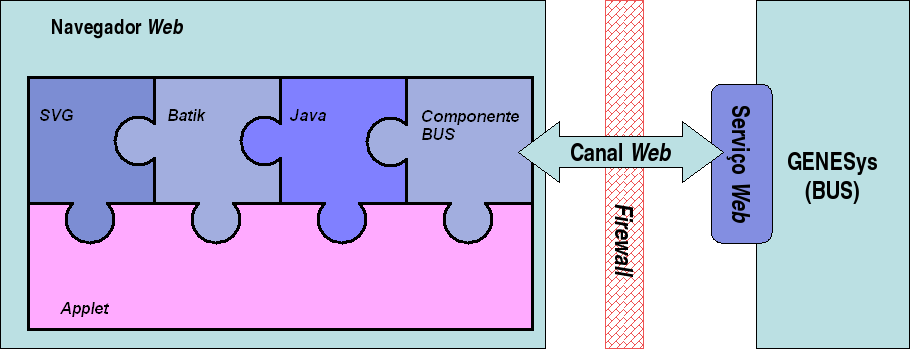
\includegraphics[width=0.86\textwidth]{puzzle}
    \caption{Arquitectura da Solução Proposta}
    \label{fig:arch}
\end{figure}

Loren ipsum dolor sit amet, consectetuer adipiscing elit. 
Praesent sit amet sem. Maecenas eleifend facilisis leo. Vestibulum et
mi. Aliquam posuere, ante non tristique consectetuer, dui elit
scelerisque augue, eu vehicula nibh nisi ac est. Suspendisse elementum
sodales felis. Nullam laoreet fermentum urna.

Duis eget diam. In est justo, tristique in, lacinia vel, feugiat eget,
quam. Pellentesque habitant morbi tristique senectus et netus et
malesuada fames ac turpis egestas. Fusce feugiat, elit ac placerat
fermentum, augue nisl ultricies eros, id fringilla enim sapien eu
felis. Vestibulum ante ipsum primis in faucibus orci luctus et
ultrices posuere cubilia Curae; Sed dolor mi, porttitor quis,
condimentum sed, luctus in. 

\subsection{Exemplo de Tabela}

É apresentado na Tabela~\ref{tab:exemplo} um exemplo de tabela
flutuante que deverá ficar no topo da página.

\begin{table}[t]
  \caption{Tabela Exemplo}
\begin{tabular}{|c|r@{.}lr@{.}lr@{.}l||r|}
	\hline
\multicolumn{8}{|c|}
	{\rule[-3mm]{0mm}{8mm}Iteração $k$ de $f(x_n)$} \\
\textbf{\em k}
	& \multicolumn{2}{c}{$x_1^k$}
	& \multicolumn{2}{c}{$x_2^k$}
	& \multicolumn{2}{c||}{$x_3^k$}
	& comentários \\ \hline \hline
0   & -0&3                 & 0&6                 &  0&7   & - \\
1   &  0&47102965 & 0&04883157 & -0&53345964  & $\delta<\epsilon$ \\
2   &  0&49988691 & 0&00228830 & -0&52246185  & $\delta < \varepsilon$ \\
3   &  0&49999976 & 0&00005380 & -0&523656   &   $N$ \\
4   &  0&5                 & 0&00000307 & -0&52359743  & \\
\vdots	& \multicolumn{2}{c}{\vdots}
	& \multicolumn{2}{c}{$\ddots$}
	& \multicolumn{2}{c||}{\vdots}  & \\
7   &  0&5   & 0&0    & \textbf{-0}&\textbf{52359878}
		 & $\delta<10^{-8}$ \\ \hline
\end{tabular}
  \label{tab:exemplo}
\end{table}

Loren ipsum dolor sit amet, consectetuer adipiscing elit. 
Praesent sit amet sem. Maecenas eleifend facilisis leo. Vestibulum et
mi. Aliquam posuere, ante non tristique consectetuer, dui elit
scelerisque augue, eu vehicula nibh nisi ac est. Suspendisse elementum
sodales felis. Nullam laoreet fermentum urna. 

Duis eget diam. In est justo, tristique in, lacinia vel, feugiat eget,
quam. Pellentesque habitant morbi tristique senectus et netus et
malesuada fames ac turpis egestas. Fusce feugiat, elit ac placerat
fermentum, augue nisl ultricies eros, id fringilla enim sapien eu
felis. Vestibulum ante ipsum primis in faucibus orci luctus et
ultrices posuere cubilia Curae; Sed dolor mi, porttitor quis,
condimentum sed, luctus in. 

\section{Secção Exemplo}

Loren ipsum dolor sit amet, consectetuer adipiscing elit. 
Praesent sit amet sem. Maecenas eleifend facilisis leo. Vestibulum et
mi. Aliquam posuere, ante non tristique consectetuer, dui elit
scelerisque augue, eu vehicula nibh nisi ac est. Suspendisse elementum
sodales felis. Nullam laoreet fermentum urna. 

\begin{lstlisting}[language=Python, caption=Python example]
# take the users input
words = input("Enter the text to translate to pig latin: ")
print(f"You entered: {words}")

# now, break apart the words into a list
words = words.split(' ')

# let's use the list to translate words greater than 3 characteres
for i in words:
    if len(i) >= 3:
        i = i + "%say" % (i[0])
        i = i[1:]
        print(i)
    else:
        pass
\end{lstlisting}

Duis eget diam. In est justo, tristique in, lacinia vel, feugiat eget,
quam. Pellentesque habitant morbi tristique senectus et netus et
malesuada fames ac turpis egestas. Fusce feugiat, elit ac placerat
fermentum, augue nisl ultricies eros, id fringilla enim sapien eu
felis. Vestibulum ante ipsum primis in faucibus orci luctus et
ultrices posuere cubilia Curae; Sed dolor mi, porttitor quis,
condimentum sed, luctus in.

\section{Resumo}

Pellentesque habitant morbi tristique senectus et netus et
malesuada fames ac turpis egestas. Fusce feugiat, elit ac placerat
fermentum, augue nisl ultricies eros, id fringilla enim sapien eu
felis. Vestibulum ante ipsum primis in faucibus orci luctus et
ultrices posuere cubilia Curae; Sed dolor mi, porttitor quis,
condimentum sed, luctus in. 

% \chapter{Mais um Capítulo}\label{chap:chap4}

Neste capítulo mostra-se apenas o formato da dissertação.

Ipsum dolor sit amet, consectetuer
adipiscing elit.  Praesent sit amet sem. 
Maecenas eleifend facilisis leo. Vestibulum et
mi. Aliquam posuere, ante non tristique consectetuer, dui elit
scelerisque augue, eu vehicula nibh nisi ac est. 
Suspendisse elementum sodales felis. 
Nullam laoreet fermentum urna. 

\section{Secção Exemplo}

Lorem ipsum dolor sit amet, consectetuer adipiscing elit. Integer
hendrerit commodo ante. Pellentesque nibh libero, aliquam at, faucibus
id, commodo a, velit. Duis eleifend sem eget leo. Morbi in
est. Suspendisse magna sem, varius nec, hendrerit non, tincidunt quis,
quam. Aenean congue. Vivamus vel est sit amet sem iaculis
posuere. Cras mollis, enim vel gravida aliquam, libero nunc
ullamcorper dui, ullamcorper sodales lectus nulla sed urna. Morbi
aliquet porta risus. Proin vestibulum ligula a purus. Maecenas a
nulla. Maecenas mattis est vitae neque auctor tempus. Etiam nulla dui,
mattis vitae, porttitor sed, aliquet ut, enim. Cras nisl magna,
aliquet et, laoreet at, gravida ac, neque. Sed id est. Nulla dapibus
dolor quis ipsum rhoncus cursus. 

Etiam nisi est, dignissim sodales, fermentum id, pulvinar ac,
eros. Duis id orci. Nam pretium nisl ac augue. Ut adipiscing magna
eget est. Curabitur varius. Nulla facilisi. Pellentesque sit amet
neque ac dui accumsan blandit. Donec mauris felis, egestas sit amet,
convallis ac, dignissim quis, dolor. Maecenas cursus tortor vel
leo. Quisque tristique. Nunc augue odio, tincidunt in, dapibus sed,
ultricies sit amet, lorem. In hac habitasse platea dictumst. Praesent
iaculis, lacus hendrerit tempor sodales, libero tellus aliquet orci,
ut rhoncus massa lectus quis erat. Pellentesque quis dolor nec tortor
rhoncus convallis. Aliquam erat volutpat. Fusce placerat, magna eu
imperdiet lobortis, augue massa blandit turpis, a consectetuer quam
arcu sit amet risus. Suspendisse potenti. Praesent sapien metus,
interdum vitae, fermentum id, faucibus ut, lorem. Nunc iaculis purus
id tortor. Aenean risus pede, laoreet ac, tristique sed, lobortis in,
turpis (see Figure~\ref{fig:2figs-b}). 

\begin{figure}
  \subfloat[UP at the left]{\label{fig:2figs-a}
    {
\includegraphics[width=5cm]{uporto-feup}}
  }
  \qquad
  \subfloat[UP at the right]{\label{fig:2figs-b}
    {
\includegraphics[width=5cm]{uporto-feup}}
  }
  \caption{Two Figures side by side}
  \label{fig:2figs}
\end{figure}

Vestibulum et lorem in ligula viverra pharetra. Curabitur quis purus
in urna facilisis bibendum. Pellentesque at arcu accumsan velit
bibendum ornare. Praesent massa. Quisque dolor. In libero. Vestibulum
ac diam id leo feugiat blandit. Donec porta, tellus ac pellentesque
molestie, felis mauris viverra lacus, sed dignissim purus justo eu
justo. Proin iaculis, nunc eu volutpat volutpat, libero purus rutrum
enim, id euismod lacus lorem nec augue. Donec hendrerit lacinia
ante. Integer mollis vulputate orci. In pellentesque, metus pharetra
elementum pharetra, est purus bibendum turpis, eu pretium sapien
libero convallis odio. Cras sodales bibendum risus. Sed mattis nulla
non leo. Nulla nunc. Phasellus egestas sodales massa. Class aptent
taciti sociosqu ad litora torquent per conubia nostra, per inceptos
himenaeos. Pellentesque habitant morbi tristique senectus et netus et
malesuada fames ac turpis egestas. Etiam mi. 

\section{Mais uma Secção}

Lorem ipsum dolor sit amet, consectetuer adipiscing elit. Quisque
purus sapien, interdum ut, vestibulum a, accumsan ullamcorper,
erat. Mauris a magna ut leo porta imperdiet. Donec dui odio, porta in,
pretium non, semper quis, orci. Quisque erat diam, pharetra vel,
laoreet ac, hendrerit vel, enim. Donec tristique luctus risus. Fusce
dolor est, eleifend id, elementum sit amet, varius vitae, neque. Morbi
at augue. Ut sem ligula, auctor vitae, facilisis id, pharetra non,
lectus. Nulla lacus augue, aliquam eget, sollicitudin sed, hendrerit
eu, leo. Suspendisse ac tortor. Mauris at odio. Etiam vehicula. Nam
lacinia purus at nibh. Aliquam fringilla lorem ac justo. Ut nec
enim. Nunc ornare, eros eu facilisis tristique, nisl lorem lacinia
risus, non ullamcorper tellus urna et eros. Quisque eleifend tempus
metus. Nunc ipsum. 

Phasellus ullamcorper justo id risus. Nunc in leo. Mauris auctor
lectus vitae est lacinia egestas. Nulla faucibus erat sit amet lectus
varius semper. Praesent ultrices vehicula orci. Nam at metus. Aenean
eget lorem nec purus feugiat molestie. Phasellus fringilla nulla ac
risus. Aliquam elementum aliquam velit. Aenean nunc odio, lobortis id,
dictum et, rutrum ac, ipsum. Aenean tellus magna, lacinia eget,
bibendum ut, interdum sit amet, ipsum. Class aptent taciti sociosqu ad
litora torquent per conubia nostra, per inceptos himenaeos. Mauris
felis lacus, dapibus sit amet, pretium feugiat, aliquet non,
purus. Aliquam elementum, diam quis porttitor gravida, sem sapien
iaculis nulla, ut pharetra odio felis a metus. Nulla lacus ipsum,
tristique ut, dapibus sed, mollis et, justo. Vivamus non ipsum sed
ligula placerat ultrices. Maecenas dictum leo adipiscing
mauris. Vestibulum tristique, lacus a consequat suscipit, nunc dui
sollicitudin arcu, non interdum libero est eget tortor. Ut eget neque
quis leo tempor dictum. 

Quisque ullamcorper. Aliquam vel magna. Sed pulvinar dictum
ligula. Sed ultrices dolor ut turpis. Vivamus sagittis orci malesuada
arcu venenatis auctor. Proin vehicula pharetra urna. Aliquam egestas
nunc quis nisl. Donec ullamcorper. Nulla purus. Ut suscipit lacus
vitae dui. Mauris semper. Ut eget sem. Integer orci. Nam vitae dui
eget nisi placerat convallis. 

Sed id lorem. Proin gravida bibendum lacus. Sed molestie, urna quis
euismod laoreet, diam dolor dictum diam, vitae consectetuer leo ipsum
id ante. Integer eu lectus non mauris pharetra viverra. In feugiat
libero ut massa. Morbi cursus, lorem sollicitudin blandit semper,
felis magna pellentesque lacus, ut rhoncus leo neque at tellus. Sed
mattis, diam eget eleifend tincidunt, ligula eros tincidunt diam,
vitae auctor turpis est vel nunc. In eu magna. Donec dolor metus,
egestas sit amet, ultrices in, faucibus sed, lectus. Etiam est enim,
vehicula pharetra, porta non, viverra vel, nunc. Ut non sem. Etiam nec
neque. Sed rhoncus, justo id imperdiet pharetra, mi tellus accumsan
neque, vitae volutpat tortor enim in odio. Nunc porta justo a
lorem. Nulla hendrerit odio vitae dolor. Suspendisse eu nisl.  

\section{Resumo ou Conclusões}

Proin vehicula pharetra urna. Aliquam egestas
nunc quis nisl. Donec ullamcorper. Nulla purus. Ut suscipit lacus
vitae dui. Mauris semper. Ut eget sem. Integer orci. Nam vitae dui
eget nisi placerat convallis. 

% \chapter{Conclusões e Trabalho Futuro} \label{chap:concl}

Proin sed justo eu sapien eleifend elementum. Pellentesque
habitant morbi tristique senectus et netus et malesuada fames ac
turpis egestas. Vivamus quam lacus, pharetra vel, aliquam vel,
volutpat sed, nisl. 

\section{Satisfação dos Objetivos}

Lorem ipsum dolor sit amet, consectetuer adipiscing elit. Etiam non
felis sed odio rutrum ultrices. Donec tempor dolor. Vivamus justo
neque, tempus id, ullamcorper in, pharetra non, tellus. Praesent eu
orci eu dolor congue gravida. Sed eu est. Donec pulvinar, lectus et
eleifend volutpat, diam sapien sollicitudin arcu, a sagittis libero
neque et dolor. Nam ligula. Cras tincidunt lectus quis nunc. Cras
tincidunt congue turpis. Nulla pede velit, sagittis a, faucibus vitae,
porttitor nec, ante. Nulla ut arcu. Cras eu augue at ipsum feugiat
hendrerit. Proin sed justo eu sapien eleifend elementum. Pellentesque
habitant morbi tristique senectus et netus et malesuada fames ac
turpis egestas. Vivamus quam lacus, pharetra vel, aliquam vel,
volutpat sed, nisl. 

Nullam erat est, vehicula id, tempor non, scelerisque at,
tellus. Pellentesque tincidunt, ante vehicula bibendum adipiscing,
lorem augue tempor felis, in dictum massa justo sed metus. Suspendisse
placerat, mi eget molestie sodales, tortor ante interdum dui, ac
sagittis est pede et lacus. Duis sapien. Nam ornare turpis et
magna. Etiam adipiscing adipiscing ipsum. Fusce sodales nisl a
arcu. Cras massa leo, vehicula facilisis, commodo a, molestie
faucibus, metus. Suspendisse potenti. Duis sagittis. Donec porta. Sed
urna. Maecenas eros. Vivamus erat ligula, pharetra sit amet, bibendum
et, fermentum sed, dolor. Nullam eleifend condimentum nibh. Integer
leo nibh, consequat eget, mollis et, sagittis ac, felis. Duis viverra
pede in pede. Phasellus molestie placerat leo. Praesent at tellus a
augue congue molestie. Proin sed justo eu sapien eleifend
elementum. Pellentesque habitant morbi tristique senectus et netus et
malesuada fames ac turpis egestas. 

\section{Trabalho Futuro}

Lorem ipsum dolor sit amet, consectetuer adipiscing elit. Aliquam
tempor tristique risus. Suspendisse potenti. Fusce id eros. In eu
enim. Praesent commodo leo. Nullam augue. Pellentesque tellus. Integer
pulvinar purus a dui convallis consectetuer. In adipiscing, orci vitae
lacinia semper, sapien elit posuere sem, ac euismod ipsum elit tempus
urna. Aliquam erat volutpat. Nullam suscipit augue sed
felis. Phasellus faucibus accumsan est. 

Aliquam felis justo, facilisis sit amet, bibendum ut, tempus ac,
dolor. Sed malesuada. Nunc non massa. In erat. Nulla
facilisi. Phasellus blandit, est in accumsan cursus, libero augue
elementum leo, vitae auctor mauris nisl ac tortor. Cras porttitor
ornare elit. Fusce at lorem. Sed lectus tortor, vestibulum id, varius
a, condimentum nec, lectus. Maecenas in nisi et magna pretium
aliquam. Pellentesque justo elit, feugiat nec, tincidunt a, dignissim
vel, ipsum. Sed nunc. Vestibulum ante ipsum primis in faucibus orci
luctus et ultrices posuere cubilia Curae; Aliquam tempus rhoncus
leo. Donec neque quam, cursus sit amet, ultricies varius, semper non,
pede. Donec porttitor. Sed aliquet feugiat elit.  

\vspace*{12mm}

Lorem ipsum dolor sit amet, consectetuer adipiscing elit. Phasellus
tellus pede, auctor ut, tincidunt a, consectetuer in, felis. Mauris
quis dolor et neque accumsan pellentesque. Donec dui magna,
scelerisque mattis, sagittis nec, porta quis, nulla. Vivamus quis
nisl. Etiam vitae nisl in diam vehicula viverra. Sed sollicitudin
scelerisque est. Nunc dapibus. Sed urna. Nulla gravida. Praesent
faucibus, risus ac lobortis dignissim, est tortor laoreet mauris,
dictum pellentesque nunc orci tincidunt tellus. Nullam pulvinar, leo
sed vestibulum euismod, ante ligula elementum pede, sit amet dapibus
lacus tortor ac nisl. Morbi libero. Integer sed dolor ac lectus
commodo iaculis. Donec ut odio.  
 

%%----------------------------------------
%% Final materials
%%----------------------------------------

%% Bibliography
%% Comment the next command if BibTeX file not used
%% bibliography is in ``myrefs.bib''
\PrintBib{myrefs}

%% 2021-07-20: change
%% comment next 2 commands if numbered appendices are not used
\appendix
% \chapter{Lorem Ipsum} \label{ap1:Lorem}

Depois das conclusões e antes das referências bibliográficas,
apresenta-se neste anexo numerado o texto usado para preencher a
dissertação.

\section{O que é o \emph{Lorem Ipsum}?}

\emph{\textbf{Lorem Ipsum}} is simply dummy text of the printing and
typesetting industry. Lorem Ipsum has been the industry's standard
dummy text ever since the 1500s, when an unknown printer took a galley
of type and scrambled it to make a type specimen book. It has survived
not only five centuries, but also the leap into electronic
typesetting, remaining essentially unchanged. It was popularised in
the 1960s with the release of Letraset sheets containing Lorem Ipsum
passages, and more recently with desktop publishing software like
Aldus PageMaker including versions of Lorem Ipsum~\citep{kn:Lip08}. 

\section{De onde Vem o Lorem?}

Contrary to popular belief, Lorem Ipsum is not simply random text. It
has roots in a piece of classical Latin literature from 45 BC, making
it over 2000 years old. Richard McClintock, a Latin professor at
Hampden-Sydney College in Virginia, looked up one of the more obscure
Latin words, consectetur, from a Lorem Ipsum passage, and going
through the cites of the word in classical literature, discovered the
undoubtable source. Lorem Ipsum comes from sections 1.10.32 and
1.10.33 of ``de Finibus Bonorum et Malorum'' (The Extremes of Good and
Evil) by Cicero, written in 45 BC. This book is a treatise on the
theory of ethics, very popular during the Renaissance. The first line
of Lorem Ipsum, ``Lorem ipsum dolor sit amet\ldots'', comes from a line in
section 1.10.32.

The standard chunk of Lorem Ipsum used since the 1500s is reproduced
below for those interested. Sections 1.10.32 and 1.10.33 from ``de
Finibus Bonorum et Malorum'' by Cicero are also reproduced in their
exact original form, accompanied by English versions from the 1914
translation by H. Rackham.

\section{Porque se usa o Lorem?}

It is a long established fact that a reader will be distracted by the
readable content of a page when looking at its layout. The point of
using Lorem Ipsum is that it has a more-or-less normal distribution of
letters, as opposed to using ``Content here, content here'', making it
look like readable English. Many desktop publishing packages and web
page editors now use Lorem Ipsum as their default model text, and a
search for ``lorem ipsum'' will uncover many web sites still in their
infancy. Various versions have evolved over the years, sometimes by
accident, sometimes on purpose (injected humour and the like). 

\section{Onde se Podem Encontrar Exemplos?}

There are many variations of passages of Lorem Ipsum available, but
the majority have suffered alteration in some form, by injected
humour, or randomised words which don't look even slightly
believable. If you are going to use a passage of Lorem Ipsum, you need
to be sure there isn't anything embarrassing hidden in the middle of
text. All the Lorem Ipsum generators on the Internet tend to repeat
predefined chunks as necessary, making this the first true generator
on the Internet. It uses a dictionary of over 200 Latin words,
combined with a handful of model sentence structures, to generate
Lorem Ipsum which looks reasonable. The generated Lorem Ipsum is
therefore always free from repetition, injected humour, or
non-characteristic words etc. 


%% Index
%% Uncomment next command if index is required
%% don't forget to run ``makeindex thesis'' command
%\PrintIndex

\end{document}
